\section{Results}
\label{sec:results}

\paragraph{Panoptic reconstruction retraining}

We leverage our synthesized dataset to refine the training of Panoptic 3D \citep{dahnert2021panoptic}.
Initially, we pre-train the 2D encoder, depth estimation and 2D instance prediction using the ADAM optimizer \citep{kingma2014adam}, a batch size of 1 and learning rate 1e-4 for 570k iterations.

The evaluation results for our 2D model compared to the pre-trained model from \citet{dahnert2021panoptic} are presented in \cref{tab:2dresults}.
As illustrated in \cref{fig:qual_panoptic}, our approach shows performance comparable to the pre-trained model. However, it encounters challenges in generating completely clear depth results, occasionally displaying some irregularities.
Hence, we use the pre-trained version of Panoptic 3D for our remaining inference experiments.
\begin{table}
  \centering
  \begin{tabular}{@{}lccc@{}}
    \toprule
     & Depth & Box Class. & Box Regress. \\
    \midrule
    \citet{dahnert2021panoptic} & 0.23 & 3.39 & \textbf{0.092}\\
    Ours & \textbf{0.196} & \textbf{1.3} & 0.149 \\
    \bottomrule
  \end{tabular}
  \caption{Results for joint training of the 2D encoder, depth estimation and 2D instance prediction. For depth we report the $\ell_1$ distance between the predicted and ground-truth depth maps. Additionally we report the $\ell_1$ distance for the regressed 2D boxes and a CE-loss on the box classification.  }
  \label{tab:2dresults}
\end{table}

\iffalse
\begin{figure}[t]
  \centering
  \begin{subfigure}[b]{0.45\linewidth}
    \centering
    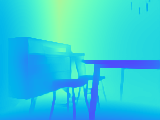
\includegraphics[width=\linewidth]{figs/depth_ours.png}
    \label{subfig:sub1}
   \vspace*{-3mm} % Adjust vertical spacing between the caption and the images
  \caption{Depth map (ours).}
  \end{subfigure}
  \hfill
  \begin{subfigure}[b]{0.45\linewidth}
    \centering
    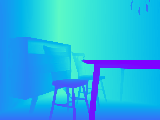
\includegraphics[width=\linewidth]{figs/depth_pan.png}
    \label{subfig:sub2}
   \vspace*{-3mm} % Adjust vertical spacing between the caption and the images
  \caption{Depth map (\citep{dahnert2021panoptic}).}
  \end{subfigure}

  \vspace{0.03\linewidth} % Adjust vertical spacing between rows of figures

  \begin{subfigure}[b]{0.45\linewidth}
    \centering
    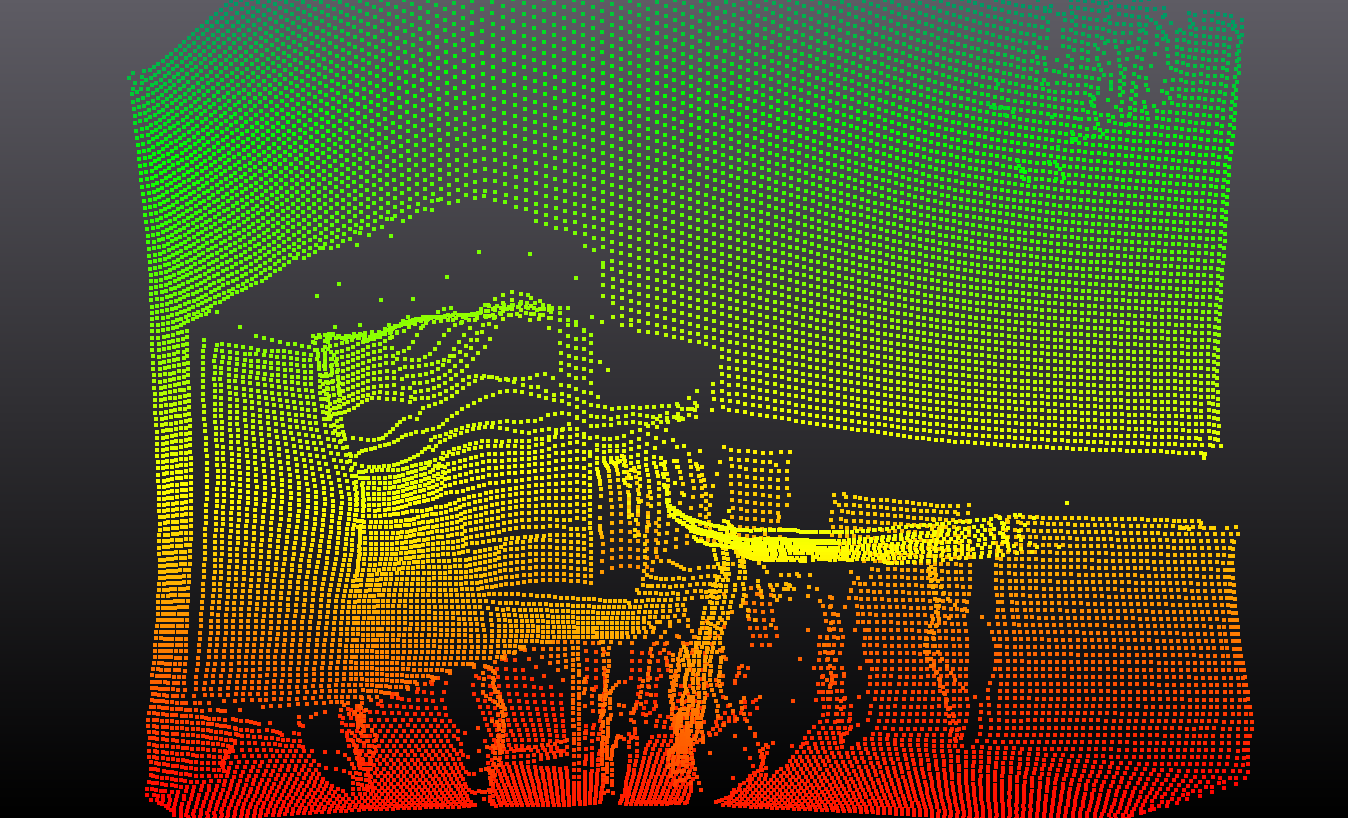
\includegraphics[width=\linewidth]{figs/depthply_ours.png}
    \label{subfig:sub3}
   \vspace*{-3mm} % Adjust vertical spacing between the caption and the images
   \caption{Geometry from depth (ours).}
  \end{subfigure}
  \hfill
  \begin{subfigure}[b]{0.45\linewidth}
    \centering
    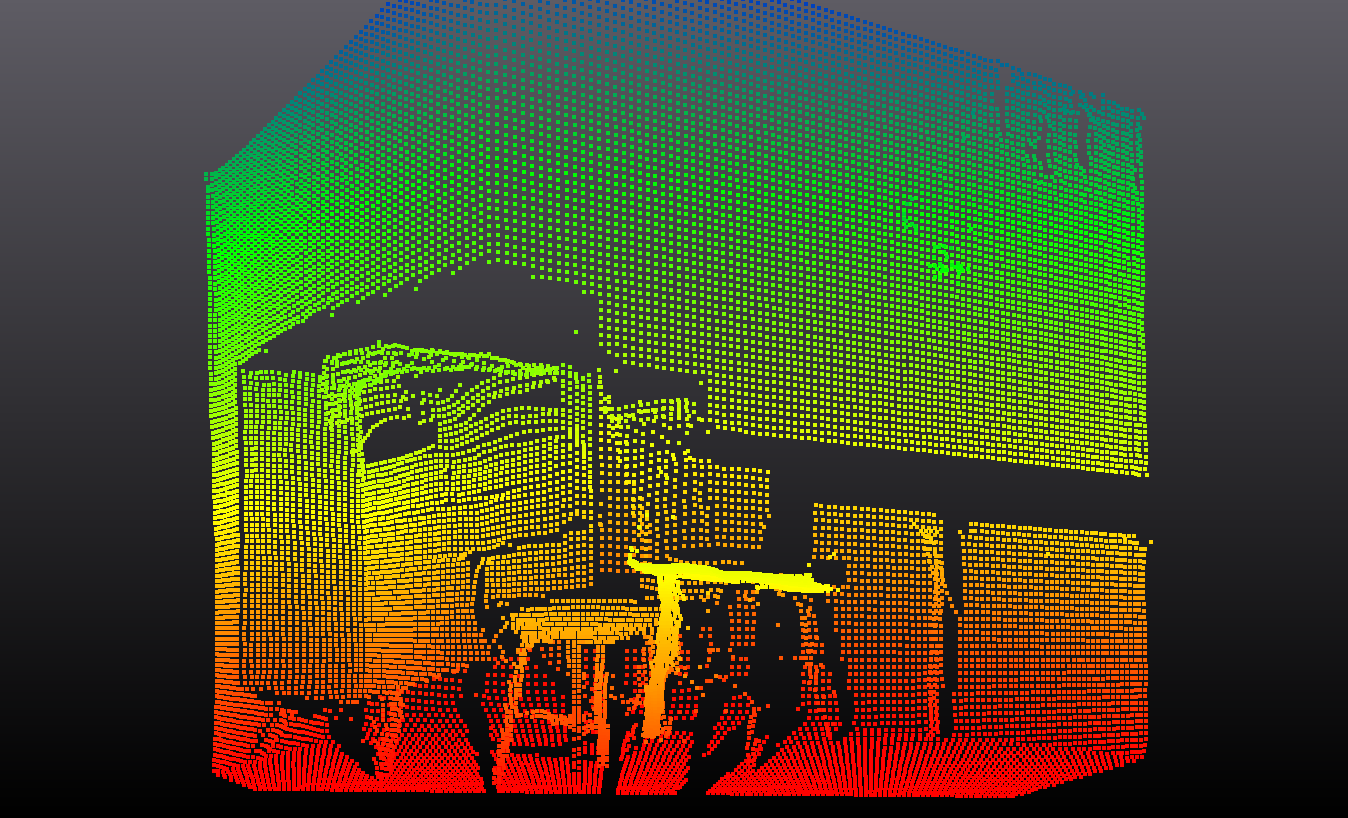
\includegraphics[width=\linewidth]{figs/depthply_pan.png}
    \label{subfig:sub4}
   \vspace*{-3mm} % Adjust vertical spacing between the caption and the images
   \caption{Geometry from depth (\citep{dahnert2021panoptic}).}
  \end{subfigure}

  \caption{2D results from the Panoptic 3D model. Our re-training results (left) vs. results from \citet{dahnert2021panoptic} (right).}
  \label{fig:qual_panoptic}
\end{figure}
\fi

\vspace*{-3mm}
\paragraph{Refined reconstruction}
\label{sec:refinedrec}

\begin{figure*}%
  \begin{subfigure}[t]{109mm}
    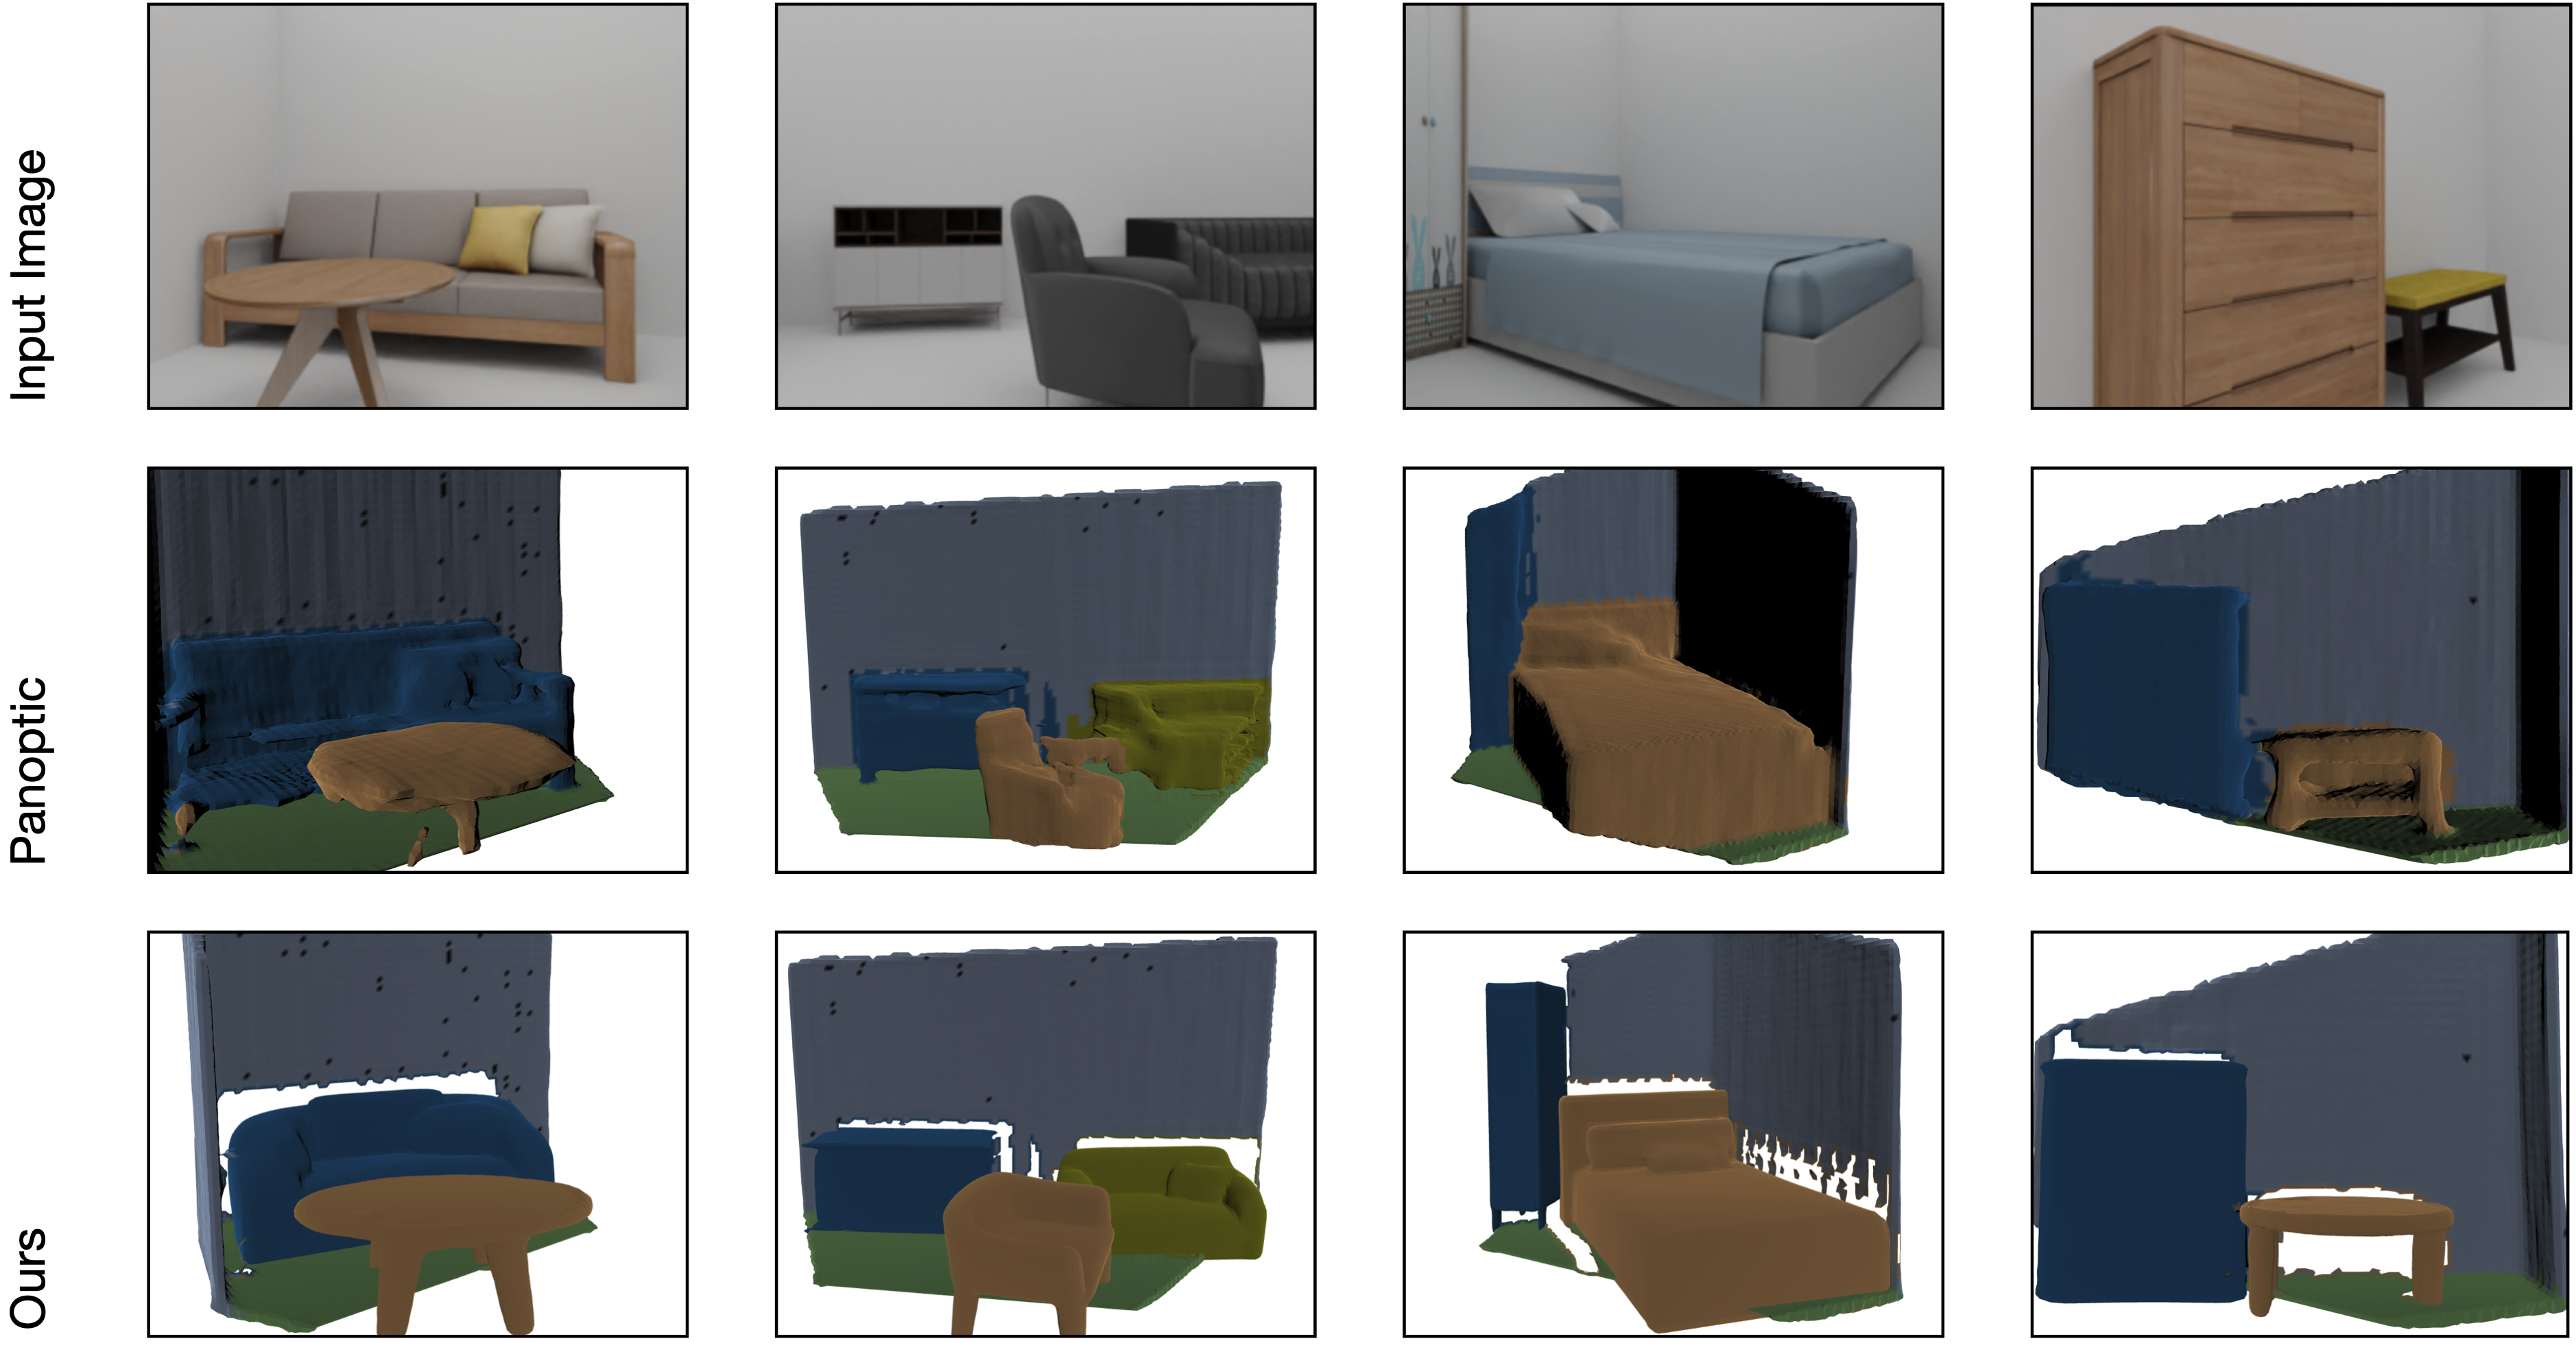
\includegraphics[width=\linewidth]{images/image1.png}
    \caption{While Panoptic 3D fails to reconstruct unobserved regions, resulting in artifacts and missing geometry, our method successfully generates complete and distinguishable 3D geometry for each instance.}\label{fig:comparison_good}
  \end{subfigure}
  \qquad
  \begin{subfigure}[t]{56mm}
    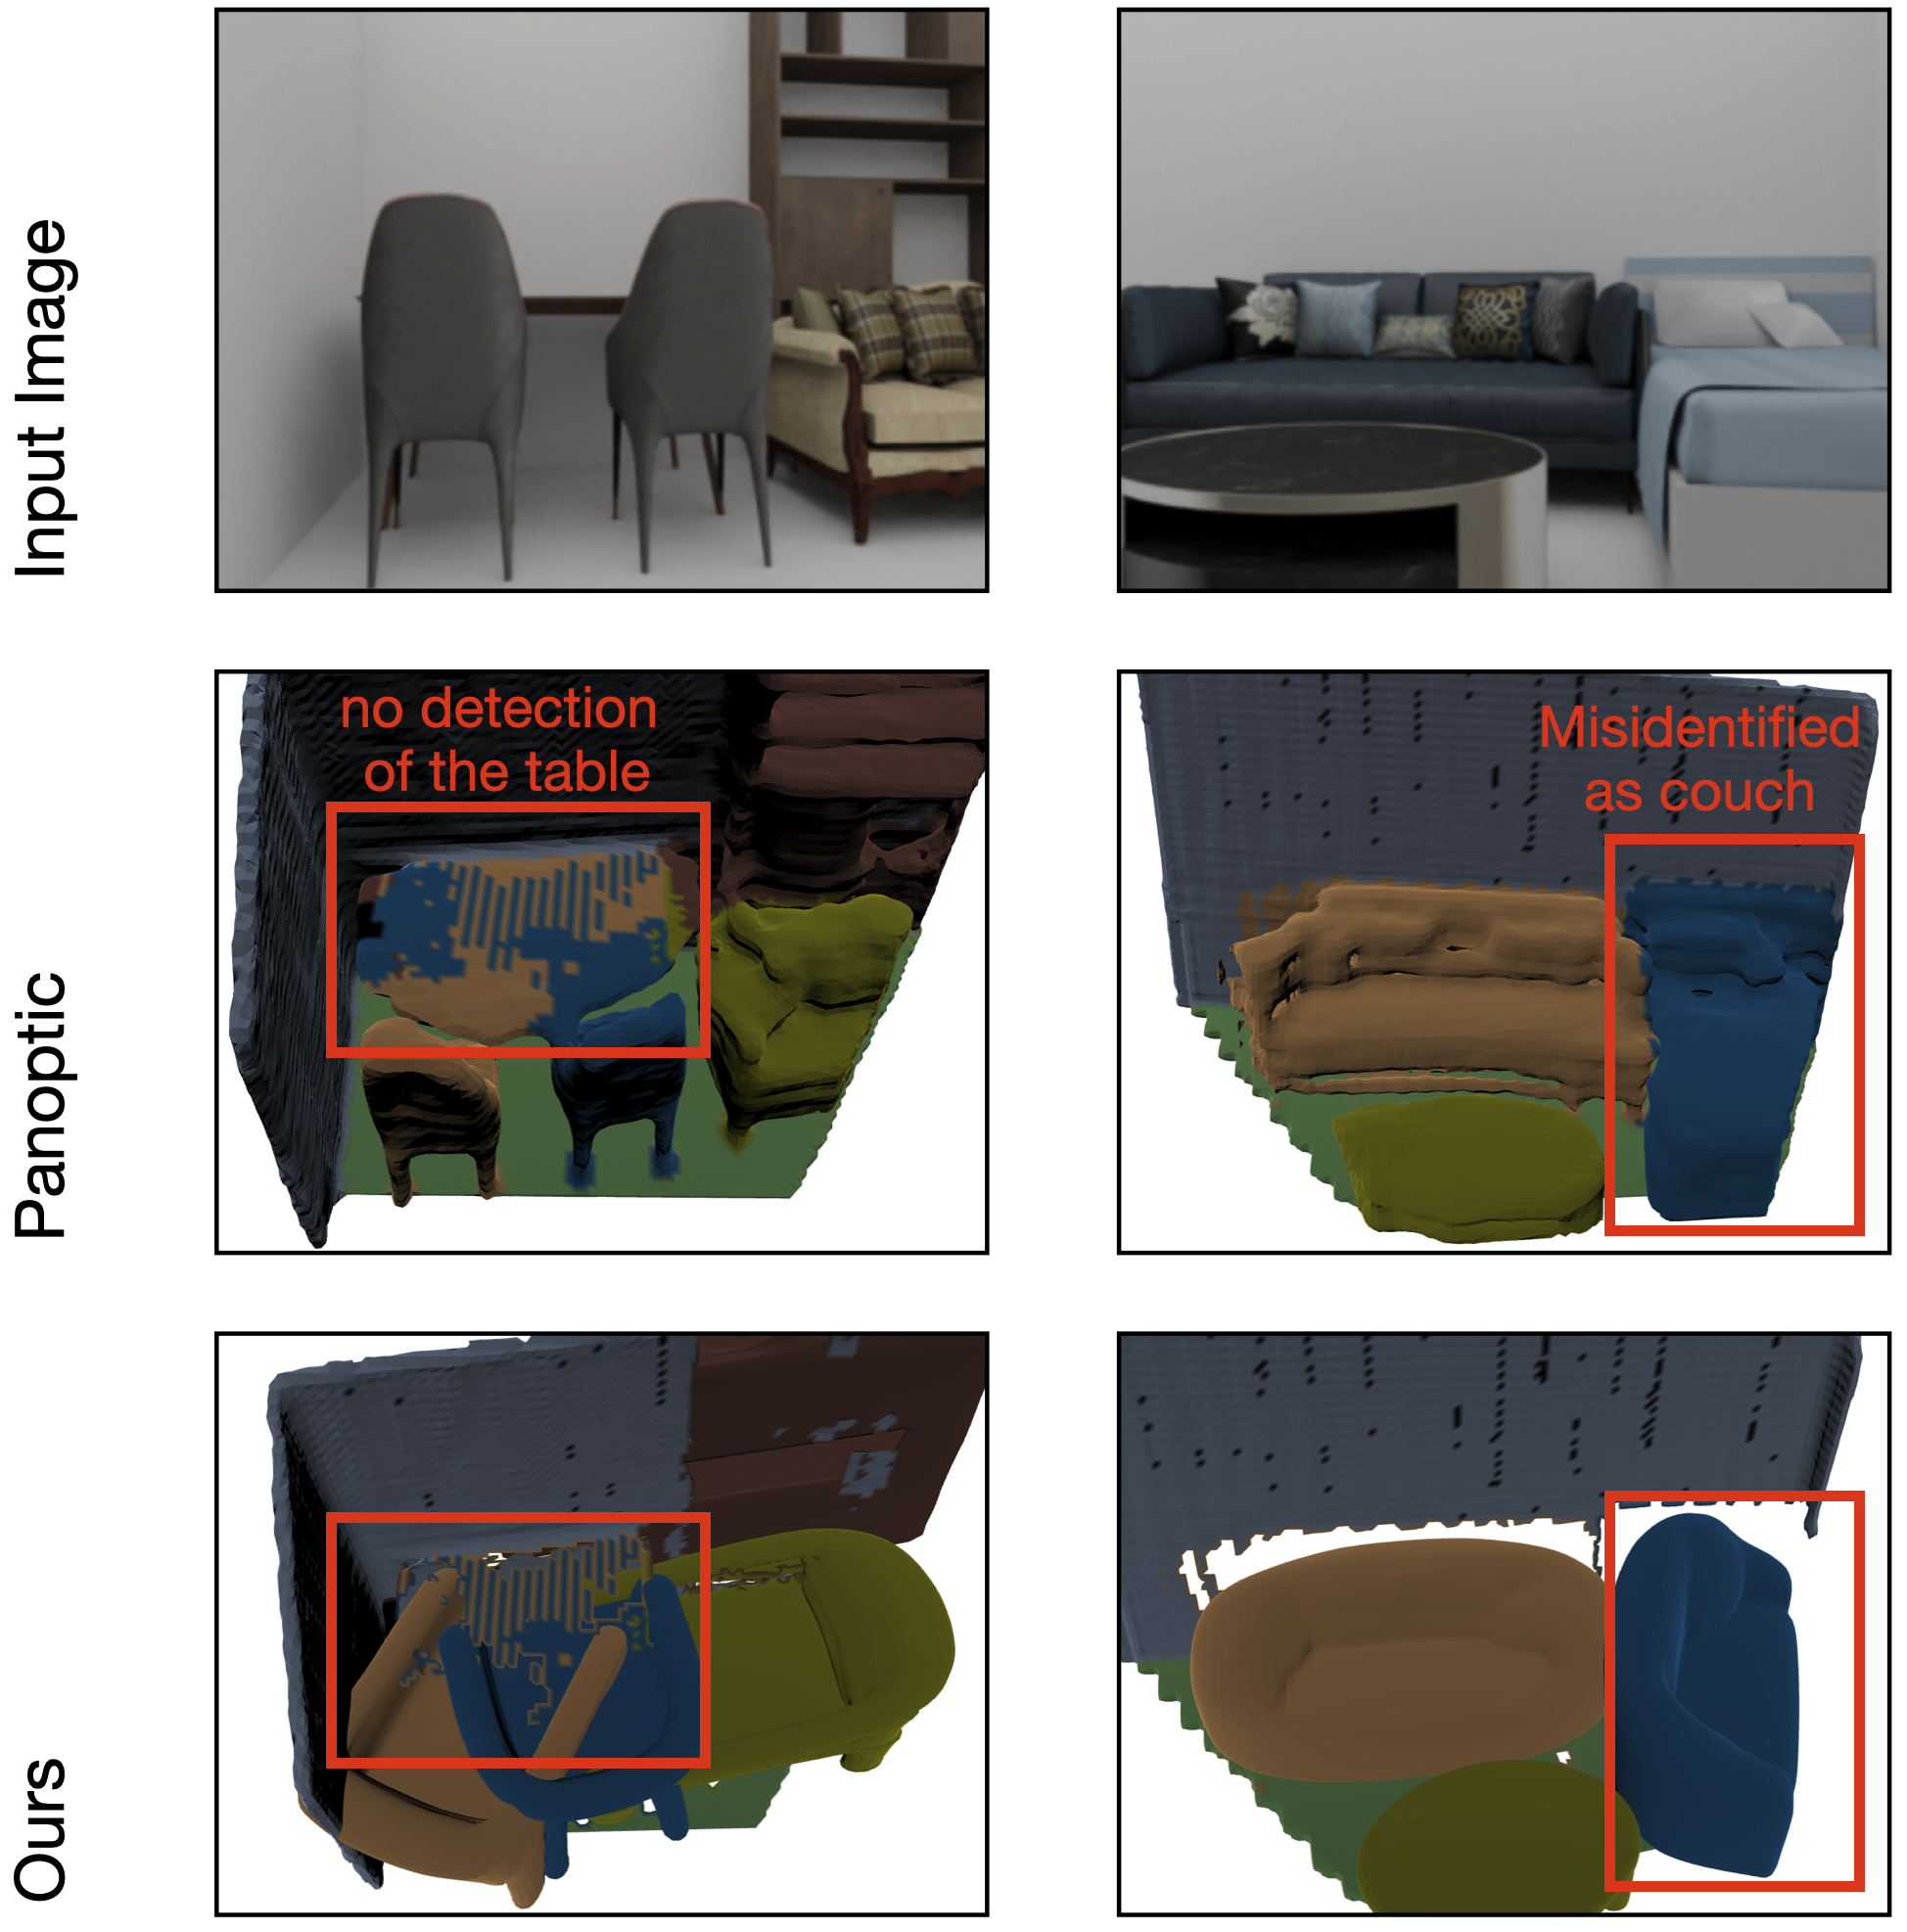
\includegraphics[width=\linewidth]{images/image2.png}
    \caption{We showcase scenarios in which our method encounters challenges in scene reconstruction. On the left, a scene is depicted where our method struggles due to missing instances, while on the right, an object is misclassified, resulting in an erroneous reconstruction.}\label{fig:comparison_bad}
  \end{subfigure}
  \caption{Comparison of pre-trained Panoptic 3D \citep{dahnert2021panoptic} vs ours.}
  \label{fig:comparison_all}
\end{figure*}

The comparison between reconstructed scenes generated by our method and those produced by Panoptic 3D is illustrated in \ref{fig:comparison_good}.
The results of Panoptic 3D exhibit instances that are noisy and lack clear edges from neighboring geometries.
Additionally, unobserved areas, whether occluded by other objects or out of sight, are disregarded, resulting in incomplete geometries within the reconstructed scene.
In contrast, our method enhances three key properties: instances have clean surfaces, are distinct from surrounding geometries, and are represented as complete objects;
all improvements which can be attributed to the incorporation of SDFusion into our inference pipeline.
In SDFusion, our approach processes each object seperately, resulting in distinct object geometries by design. Our alignment procedure yields proper placement of refined instances within the scene.

Conversely, in cases where instance mask predictions are noisy, or instances are missing completely, our method struggles to create good scene reconstructions (Figure \ref{fig:comparison_bad}). In this setting, Panoptic 3D generates the table, but is not able to identify it. Due to the absence of the table instance, SDFusion is unable to reconstruct it. For the other instances, our method can maintain smoothness even with bad-quality mask predictions, but our alignment algorithm occasionally fails, resulting in object intersections, disproportionate scales and incorrect orientations. Lastly, our method also struggles if wrong labels are provided for an instance (Figure \ref{fig:comparison_bad}).

We solely focus on qualitative results since we prioritize aesthetic quality over exact reconstruction. To obtain quantitative results in this setting, we refer to the evaluation method of \citet{wu2018learning}.
\paragraph{SDFusion fine-tuning}

In order to align SDFusion to the shape distribution of 3D-Front, we fine-tune the model on the 3D-Future dataset \citep{fu20213e}.
We examine the effects of fine-tuning SDFusion in \ref{sec:appendic_fine_tuning}.
